\documentclass{if-beamer}
\DeclareUnicodeCharacter{2212}{-}
% --------------------------------------------------- %
%                  Presentation info	              %
% --------------------------------------------------- %
\title[Lecture 10]{Lecture 10 }
\subtitle{Root Finding: Bracket Methods}
\author{Instructor: Ashley Gannon}
\date{ISC3313 Fall 2021}
\logo{

\includegraphics[scale=0.08]{figures/FSULogo.png}
}
\subject{Presentation subject}

% --------------------------------------------------- %
%                    Title + Schedule                 %
% --------------------------------------------------- %
\begin{document}

\begin{frame}
  \titlepage
\end{frame}
% --------------------------------------------------- %
%                      Presentation                   %
% --------------------------------------------------- %
\section{Roots of functions}
\begin{frame}
\frametitle{Recall the quadratic formula}
Years ago you learned the quadratic formula
$$x = \frac{-b \pm \sqrt{b^2-4ac}}{2a} $$
to solve 
$$f(x) = ax^2 +bx+c =0.$$

The values of $x$ found by using the quadratic formula are the "roots" of the above equation. The roots are the values of $x$ where $f(x)=0$.   \\
\vspace{8pt}
While the quadratic equation is handy for solving the above equation, there are many other functions where the roots cannot be determined easily. 
\begin{equation*}
a_{n} x^{n} + a_{n-1} x^{n-1} \dots a_{1} x + a_{0} = 0
\end{equation*}
\end{frame}

\begin{frame}
\frametitle{Recall the quadratic formula}
Years ago you learned the quadratic formula
$$x = \frac{-b \pm \sqrt{b^2-4ac}}{2a} $$
to solve 
$$f(x) = ax^2 +bx+c =0.$$

The values of $x$ found by using the quadratic formula are the "roots" of the above equation. The roots are the values of $x$ where $f(x)=0$.   \\
\vspace{8pt}
While the quadratic equation is handy for solving the above equation, there are many other functions where the root cannot be determined easily. 
\begin{equation*}
a_{n} x^{n} + a_{n-1} x^{n-1} \dots a_{1} x + a_{0} = 0
\end{equation*}
Before digital computers were around, people found the roots of a function often one of two ways. They either used a direct method, like the quadratic formula, or an approximate solution technique, such as by plotting the function and approximating where the function crosses the x-axis or by guessing where the function is equal to 0. 
\end{frame}


\begin{frame}
\frametitle{Approximate techniques}
Given a function $f(x)$, we consider the problem of finding the point $x = x^{*}$ (the
\textit{root}) such that the equation
\begin{equation*}
f(x) = 0
\end{equation*}
is satisfied. Given a domain, the equation may have multiple solutions, one
solution, or no solutions.  Consider the following example:
\begin{figure}
	\center
	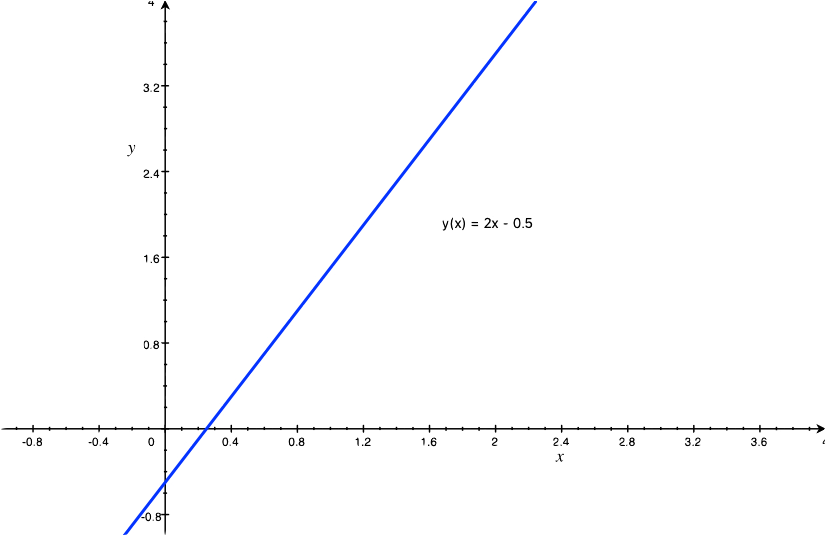
\includegraphics[width=0.6\textwidth]{figures/linear}
\end{figure}
How many roots does this equation have? What's the approximate value?
\end{frame}

\begin{frame}
\frametitle{Approximate techniques}
Given a function $f(x)$, we consider the problem of finding the point $x = x^{*}$ (the
\textit{root}) such that the equation
\begin{equation*}
f(x) = 0
\end{equation*}
is satisfied. Given a domain, the equation may have multiple solutions, one
solution, or no solutions.  Consider the following example:
\begin{figure}
	\center
	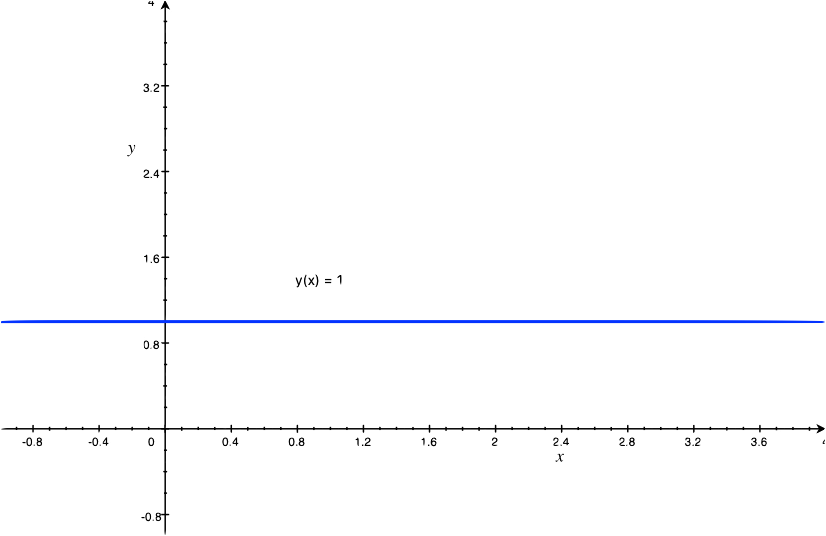
\includegraphics[width=0.6\textwidth]{figures/const}
\end{figure}
How many roots does this equation have? What is the approximate value? 
\end{frame}

\begin{frame}
\frametitle{Approximate techniques}
Given a function $f(x)$, we consider the problem of finding the point $x = x^{*}$ (the
\textit{root}) such that the equation
\begin{equation*}
f(x) = 0
\end{equation*}
is satisfied. Given a domain, the equation may have multiple solutions, one
solution, or no solutions.  Consider the following example:
\begin{figure}
	\center
	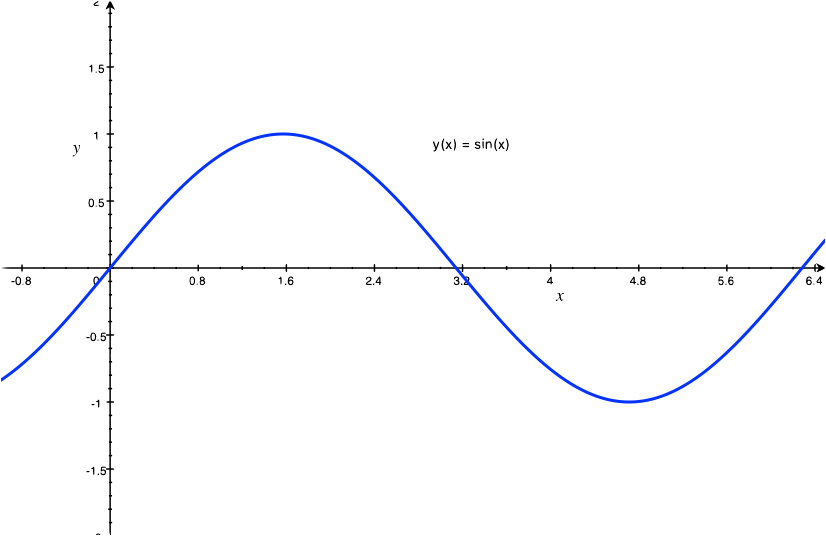
\includegraphics[width=0.6\textwidth]{figures/sin}
\end{figure}
How many roots does this equation have? What is the approximate value? 
\end{frame}

\begin{frame}
\frametitle{Approximate techniques}
Here we zoom out a little on the sine function...
\begin{figure}
\center
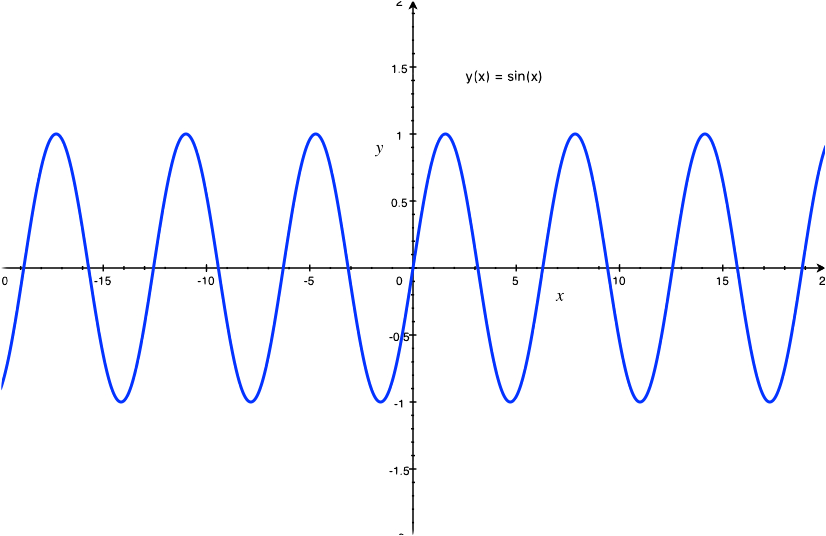
\includegraphics[width=0.75\textwidth]{figures/bigsin.png}
\end{figure}
\end{frame}

\begin{frame}
\frametitle{Approximate techniques}
Not all examples are so trivial. Consider this problem:\\
\vspace{10pt}
Medical studies have established that a bungee jumper’s chances of sustaining a significant vertebrae injury increase significantly if the free-fall velocity exceeds 36 m/s after 4 s of free fall. Your boss at the bungee-jumping company wants you to determine the mass at which this criterion is exceeded given a drag coefficient of 0.25 kg/m. \\
\vspace{10pt}
You know from your previous studies that the following analytical solution can be used to predict fall velocity as a function of time:
$$v(t)= \sqrt{\frac{gm}{c_d}}\tanh\left(\sqrt{\frac{gc_d}{m}}t\right)  $$
\end{frame}

\begin{frame}
\frametitle{Approximate techniques}
Not all examples are so trivial. Consider this problem:\\
\vspace{10pt}
Medical studies have established that a bungee jumper’s chances of sustaining a significant vertebrae injury increase significantly if the free-fall velocity exceeds 36 m/s after 4 s of free fall. Your boss at the bungee-jumping company wants you to determine the mass at which this criterion is exceeded given a drag coefficient of 0.25 kg/m. \\
\vspace{10pt}
You know from your previous studies that the following analytical solution can be used to predict fall velocity as a function of time:
$$v(t)= \sqrt{\frac{gm}{c_d}}\tanh\left(\sqrt{\frac{gc_d}{m}}t\right)  $$
Try as you might, you cannot manipulate this equation to explicitly solve for m—that is, you cannot isolate the mass on the left side of the equation.
\end{frame}

\begin{frame}
\frametitle{Approximate techniques}
An alternative way of looking at the problem involves subtracting $v(t)$ from both sides to give a new function:
$$f(m) = \sqrt{\frac{gm}{c_d}}\tanh\left(\sqrt{\frac{gc_d}{m}}t\right) -v(t) $$
Now we can see that the answer to the problem is the value of $m$ that makes the function $f(m)$ equal to zero.
\end{frame}

\begin{frame}
\frametitle{Approximate techniques}
Use the graphical approach to determine the mass of the bungee jumper with a drag coefficient of $c_d = 0.25 kg/m$, a velocity of $v(t)=36 m/s$ after $t = 4 s$ of free fall. Note: The acceleration of gravity $g \approx 9.81 m/s^2$
\begin{figure}
	\centering
	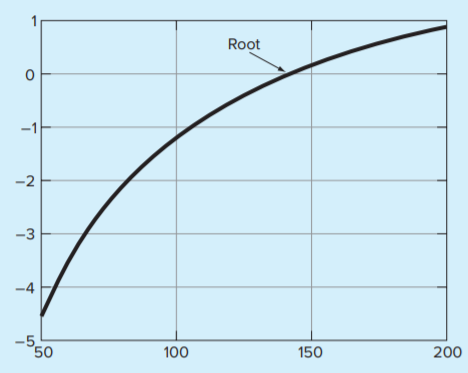
\includegraphics[width = 0.6\textwidth]{figures/BunjeeJumpGraph}
\end{figure}
 What is the approximate value? 
\end{frame}

\begin{frame}
\frametitle{Approximate techniques}
Use the graphical approach to determine the mass of the bungee jumper with a drag coefficient of $c_d = 0.25 kg/m$, a velocity of $v(t)=36 m/s$ after $t = 4 s$ of free fall. Note: The acceleration of gravity $g \approx 9.81 m/s^2$ \\
\vspace{5pt}
\begin{minipage}{0.5\textwidth}
	\begin{figure}
		\centering
		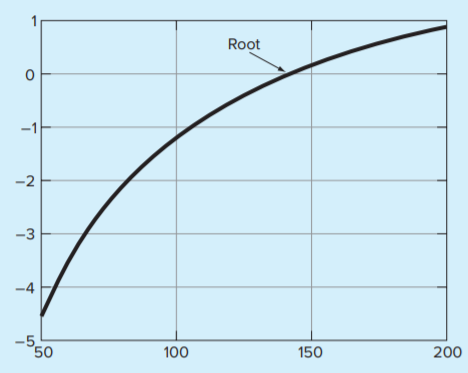
\includegraphics[width = \textwidth]{figures/BunjeeJumpGraph}
	\end{figure}
\end{minipage}
\begin{minipage}{0.5\textwidth}
	The function crosses the x axis between $m= 140 kg$ and $m=150 kg$. Visual inspection of the plot provides a rough estimate of the root of $m=145 kg$ (about 320 lb). The validity of the graphical estimate can be checked by substituting it into our equation
	$$f(m) = \sqrt{\frac{gm}{c_d}}\tanh\left(\sqrt{\frac{gc_d}{m}}t\right) -v(t) $$
	which gives us a value close to 0.
\end{minipage}
\end{frame}

\begin{frame}
\frametitle{Approximate techniques}
Use the graphical approach to determine the mass of the bungee jumper with a drag coefficient of $c_d = 0.25 kg/m$, a velocity of $v(t)=36 m/s$ after $t = 4 s$ of free fall. Note: The acceleration of gravity $g \approx 9.81 m/s^2$ \\
\vspace{5pt}
\begin{minipage}{0.5\textwidth}
	\begin{figure}
		\centering
		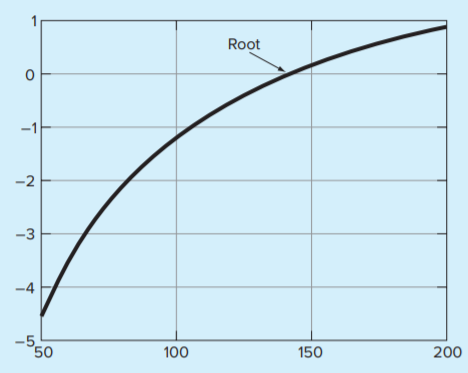
\includegraphics[width = \textwidth]{figures/BunjeeJumpGraph}
	\end{figure}
\end{minipage}
\begin{minipage}{0.5\textwidth}
	The function crosses the x axis between $m= 140 kg$ and $m=150 kg$. Visual inspection of the plot provides a rough estimate of the root of $m=145 kg$ (about 320 lb). The validity of the graphical estimate can be checked by substituting it into our equation
	$$f(m) = \sqrt{\frac{gm}{c_d}}\tanh\left(\sqrt{\frac{gc_d}{m}}t\right) -v(t) $$
	which gives us a value close to 0.
\end{minipage}
$$0.0456\approx \sqrt{\frac{9.81*145}{0.25}}\tanh\left(\sqrt{\frac{9.81*0.25}{145}}*4\right) -36 $$
\end{frame}

\begin{frame}
\frametitle{Approximate techniques}
Use the graphical approach to determine the mass of the bungee jumper with a drag coefficient of $c_d = 0.25 kg/m$, a velocity of $v(t)=36 m/s$ after $t = 4 s$ of free fall. Note: The acceleration of gravity $g \approx 9.81 m/s^2$ \\
\vspace{5pt}
\begin{minipage}{0.5\textwidth}
	\begin{figure}
		\centering
		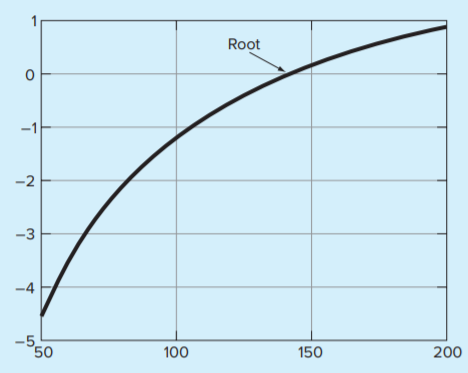
\includegraphics[width = \textwidth]{figures/BunjeeJumpGraph}
	\end{figure}
\end{minipage}
\begin{minipage}{0.5\textwidth}
	It can also be checked by substituting it into
	$$v(t) = \sqrt{\frac{gm}{c_d}}\tanh\left(\sqrt{\frac{gc_d}{m}}t\right)$$
	which gives us a value close to 36.
\end{minipage}

\end{frame}

\begin{frame}
\frametitle{Approximate techniques}
Use the graphical approach to determine the mass of the bungee jumper with a drag coefficient of $c_d = 0.25 kg/m$, a velocity of $v(t)=36 m/s$ after $t = 4 s$ of free fall. Note: The acceleration of gravity $g \approx 9.81 m/s^2$ \\
\vspace{5pt}
\begin{minipage}{0.5\textwidth}
	\begin{figure}
		\centering
		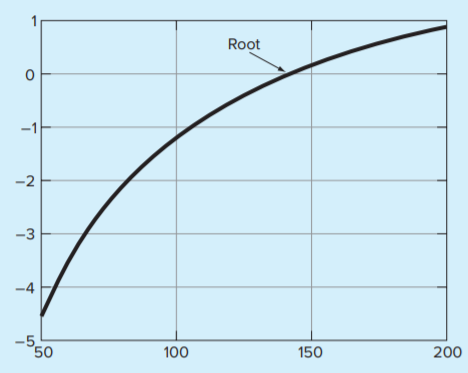
\includegraphics[width = \textwidth]{figures/BunjeeJumpGraph}
	\end{figure}
\end{minipage}
\begin{minipage}{0.5\textwidth}
	It can also be checked by substituting it into
	$$v(t) = \sqrt{\frac{gm}{c_d}}\tanh\left(\sqrt{\frac{gc_d}{m}}t\right)$$
	which gives us a value close to 36.
\end{minipage}
$$36.0456\approx \sqrt{\frac{9.81*145}{0.25}}\tanh\left(\sqrt{\frac{9.81*0.25}{145}}*4\right) $$
\end{frame}

\begin{frame}
Sure, you can keep guessing values and substituting them in to get closer to the root, or closer to the desired velocity. Depending on what you want your error to be, this could be very time consuming. \\
\vspace{10pt}
But the big question is: How confident would you be telling your boss that the maximum cutoff weight for this bungee jump is 145 kg/ 320lbs? Knowing that if your estimate is off, someone could be seriously injured.
\end{frame}

\begin{frame}
\frametitle{Approximate techniques}
These methods are haphazard at best, lack precision, and are just overall inefficient if the roots aren't obvious. However, they can be utilized to obtain rough estimates of roots. These estimates can be employed as starting guesses for numerical methods. They can also be used to tell when a numerical method might fail.\\
\vspace{10pt}
Numerical methods present alternatives that are also approximate solutions, but employ systematic strategies that home in on a true root. Using these systemic algorithms to find the root(s) of an equations is a simple and efficient task.\\
\vspace{10pt}
In this section of the course we will cover:
\begin{itemize}
	\item Bracketing methods: These methods are based on two initial guesses that "bracket" the root - they are on either side of the root.  
	\begin{itemize}
		\item Incremental search
		\item Bisection
	\end{itemize}
	\item Open methods: These methods can involve one or more initial guesses, but they do not bracket the root.
	\begin{itemize}
		\item Simple fixed-point iteration
		\item Newton-Raphson
		\item Secant method
	\end{itemize}
\end{itemize}  
\end{frame}

\begin{frame}
\frametitle{Approximate techniques}
Similarities and differences between bracketed and open methods: \\
\vspace{10pt}
\begin{itemize}
	\item For well-posed problems, the bracketing methods always work but converge slowly (i.e., they typically take more iterations to home in on the answer). In contrast, the open methods do not always work (i.e., they can diverge). But when they do work, they usually converge quicker. \\\vspace{10pt}
\end{itemize}

\end{frame}

\begin{frame}
\frametitle{Approximate techniques}
Similarities and differences between bracketed and open methods: \\
\vspace{10pt}
\begin{itemize}
	\item For well-posed problems, the bracketing methods always work but converge slowly (i.e., they typically take more iterations to home in on the answer). In contrast, the open methods do not always work (i.e., they can diverge). But when they do work, they usually converge quicker. \\\vspace{10pt}
	\item In both cases, initial guesses are required. These may naturally arise from the physical context you are analyzing, or they may not be obvious at all.
\end{itemize}
\end{frame}


\section{What makes a problem "well-posed"?}
\begin{frame}
\frametitle{A well-posed problem}
The term \textit{"well-posed problem"} describes mathematical models of physical phenomena should have the properties that:
\begin{itemize}
	\item a solution exists,
\end{itemize}

\end{frame}

\begin{frame}
\frametitle{A well-posed problem}
The term \textit{"well-posed problem"} describes mathematical models of physical phenomena should have the properties that:
\begin{itemize}
	\item a solution exists,
	\item the solution is unique,
\end{itemize}

\end{frame}

\begin{frame}
\frametitle{A well-posed problem}
The term \textit{"well-posed problem"} describes mathematical models of physical phenomena should have the properties that:
\begin{itemize}
	\item a solution exists,
	\item the solution is unique,
	\item the solution's behavior changes continuously
\end{itemize}
\end{frame}


\begin{frame}
\frametitle{Continuous functions}
If $f$ is a function defined on an interval $[a,b]$, and we have a
point $c \in [a,b]$, then $f$ is continuous at $c$ if
\begin{equation*}
\lim_{x \rightarrow c} f(x) = f(c)
\end{equation*}
In other words, as $x$ gets closer and closer to $c$ then $f(x)$ gets closer and closer to $f(c)$. And we have to check this condition from the left and the right of $c$.
\end{frame}

\begin{frame}
\frametitle{Continuous functions}
If $f$ is a function defined on an interval $[a,b]$, and we have a
point $c \in [a,b]$, then $f$ is continuous at $c$ if
\begin{equation}
\lim_{x \rightarrow c} f(x) = f(c)
\end{equation}
In other words, as $x$ gets closer and closer to $c$ then $f(x)$ gets closer and closer to $f(c)$. And we have to check this condition from the left and the right of $c$. \\
\vspace{10pt}
\begin{minipage}{0.5\textwidth}
	From the left:
	\centering
	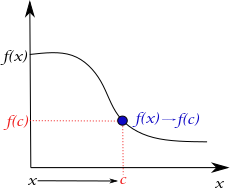
\includegraphics[width = 0.8\textwidth]{figures/left}
\end{minipage}
\end{frame}

\begin{frame}
\frametitle{Continuous functions}
If $f$ is a function defined on an interval $[a,b]$, and we have a
point $c \in [a,b]$, then $f$ is continuous at $c$ if
\begin{equation}
\lim_{x \rightarrow c} f(x) = f(c)
\end{equation}
In other words, as $x$ gets closer and closer to $c$ then $f(x)$ gets closer and closer to $f(c)$. And we have to check this condition from the left and the right of $c$. \\
\vspace{10pt}
\begin{minipage}{0.5\textwidth}
	From the left:
	\centering
	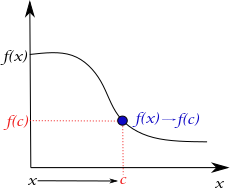
\includegraphics[width = 0.8\textwidth]{figures/left}
\end{minipage}
\begin{minipage}{0.5\textwidth}
	From the right:
	\centering
	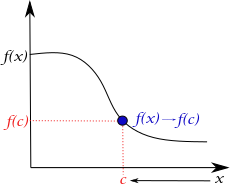
\includegraphics[width = 0.8\textwidth]{figures/right}
\end{minipage}
\end{frame}

\begin{frame}
\frametitle{Continuous functions}
If $f$ is a function defined on an interval $[a,b]$, and we have a
point $c \in [a,b]$, then $f$ is continuous at $c$ if
\begin{equation}
\lim_{x \rightarrow c} f(x) = f(c)
\end{equation}
In other words, as $x$ gets closer and closer to $c$ then $f(x)$ gets closer and closer to $f(c)$. And we have to check this condition from the left and the right of $c$. \\
\vspace{10pt}
\begin{minipage}{0.5\textwidth}
	From the left:
	\centering
	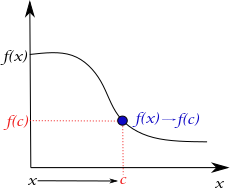
\includegraphics[width = 0.8\textwidth]{figures/left}
\end{minipage}
\begin{minipage}{0.5\textwidth}
	From the right:
	\centering
	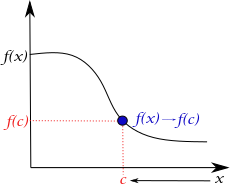
\includegraphics[width = 0.8\textwidth]{figures/right}
\end{minipage}
\end{frame}

\begin{frame}
\frametitle{Continuous functions}
\begin{minipage}{0.5\textwidth}
	From the left:
	\centering
	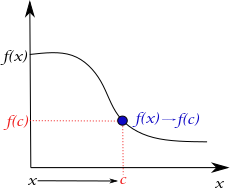
\includegraphics[width = 0.8\textwidth]{figures/left}
\end{minipage}
\begin{minipage}{0.5\textwidth}
	From the right:
	\centering
	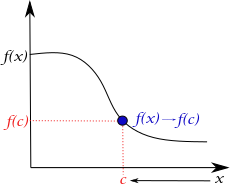
\includegraphics[width = 0.8\textwidth]{figures/right}
\end{minipage}
\\\vspace{10pt}
If we get different values from left and right (a "jump"), then...
\begin{figure}
	\centering
	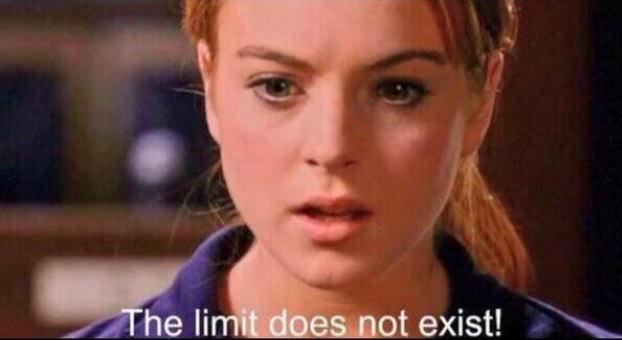
\includegraphics[width = 0.35\textwidth]{figures/limitdne}
\end{figure} 

If for every point on the interval the limit exists, then the function is continuous on the interval.
\end{frame}

\begin{frame}
\frametitle{Continuous functions}
Is the function below continuous on the whole interval shown?
\begin{figure}
\center
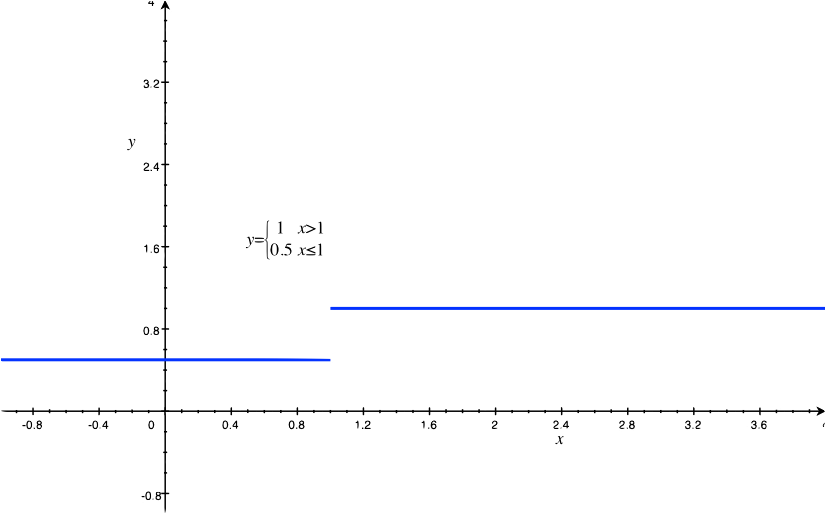
\includegraphics[width=0.75\textwidth]{figures/disc.png}
\end{figure}
\end{frame}

\begin{frame}
\frametitle{Intermediate value theorem}
Functions that are continuous on the interval [a,b] exhibit many useful properties. One powerful theorem concerning such functions is the \textbf{intermediate value theorem}. This method is useful for finding roots of such a function, i.e. a solution to our root finding problem.\\\vspace{5pt} 

\end{frame}

\begin{frame}
\frametitle{Intermediate value theorem}
Functions that are continuous on the interval [a,b] exhibit many useful properties. One powerful theorem concerning such functions is the \textbf{intermediate value theorem}. This method is useful for finding roots of such a function, i.e. a solution to our root finding problem.\\\vspace{5pt} 
The intermediate value theorem states that if $f$ is a continuous function
on the interval $[a,b]$,  then it takes on any value between
$f(a)$ and $f(b)$ at some point within the interval. In other words,
let $s$ be a number with $f(a) < s < f(b)$. Then there exists some
$x$ such that $f(x) = s$. \\
\vspace{10pt}
In this example, we see that for some value $f(a) < s < f(b)$, there are several such $x$ values that satisfy $f(x) = s$.
\begin{figure}
	\center
	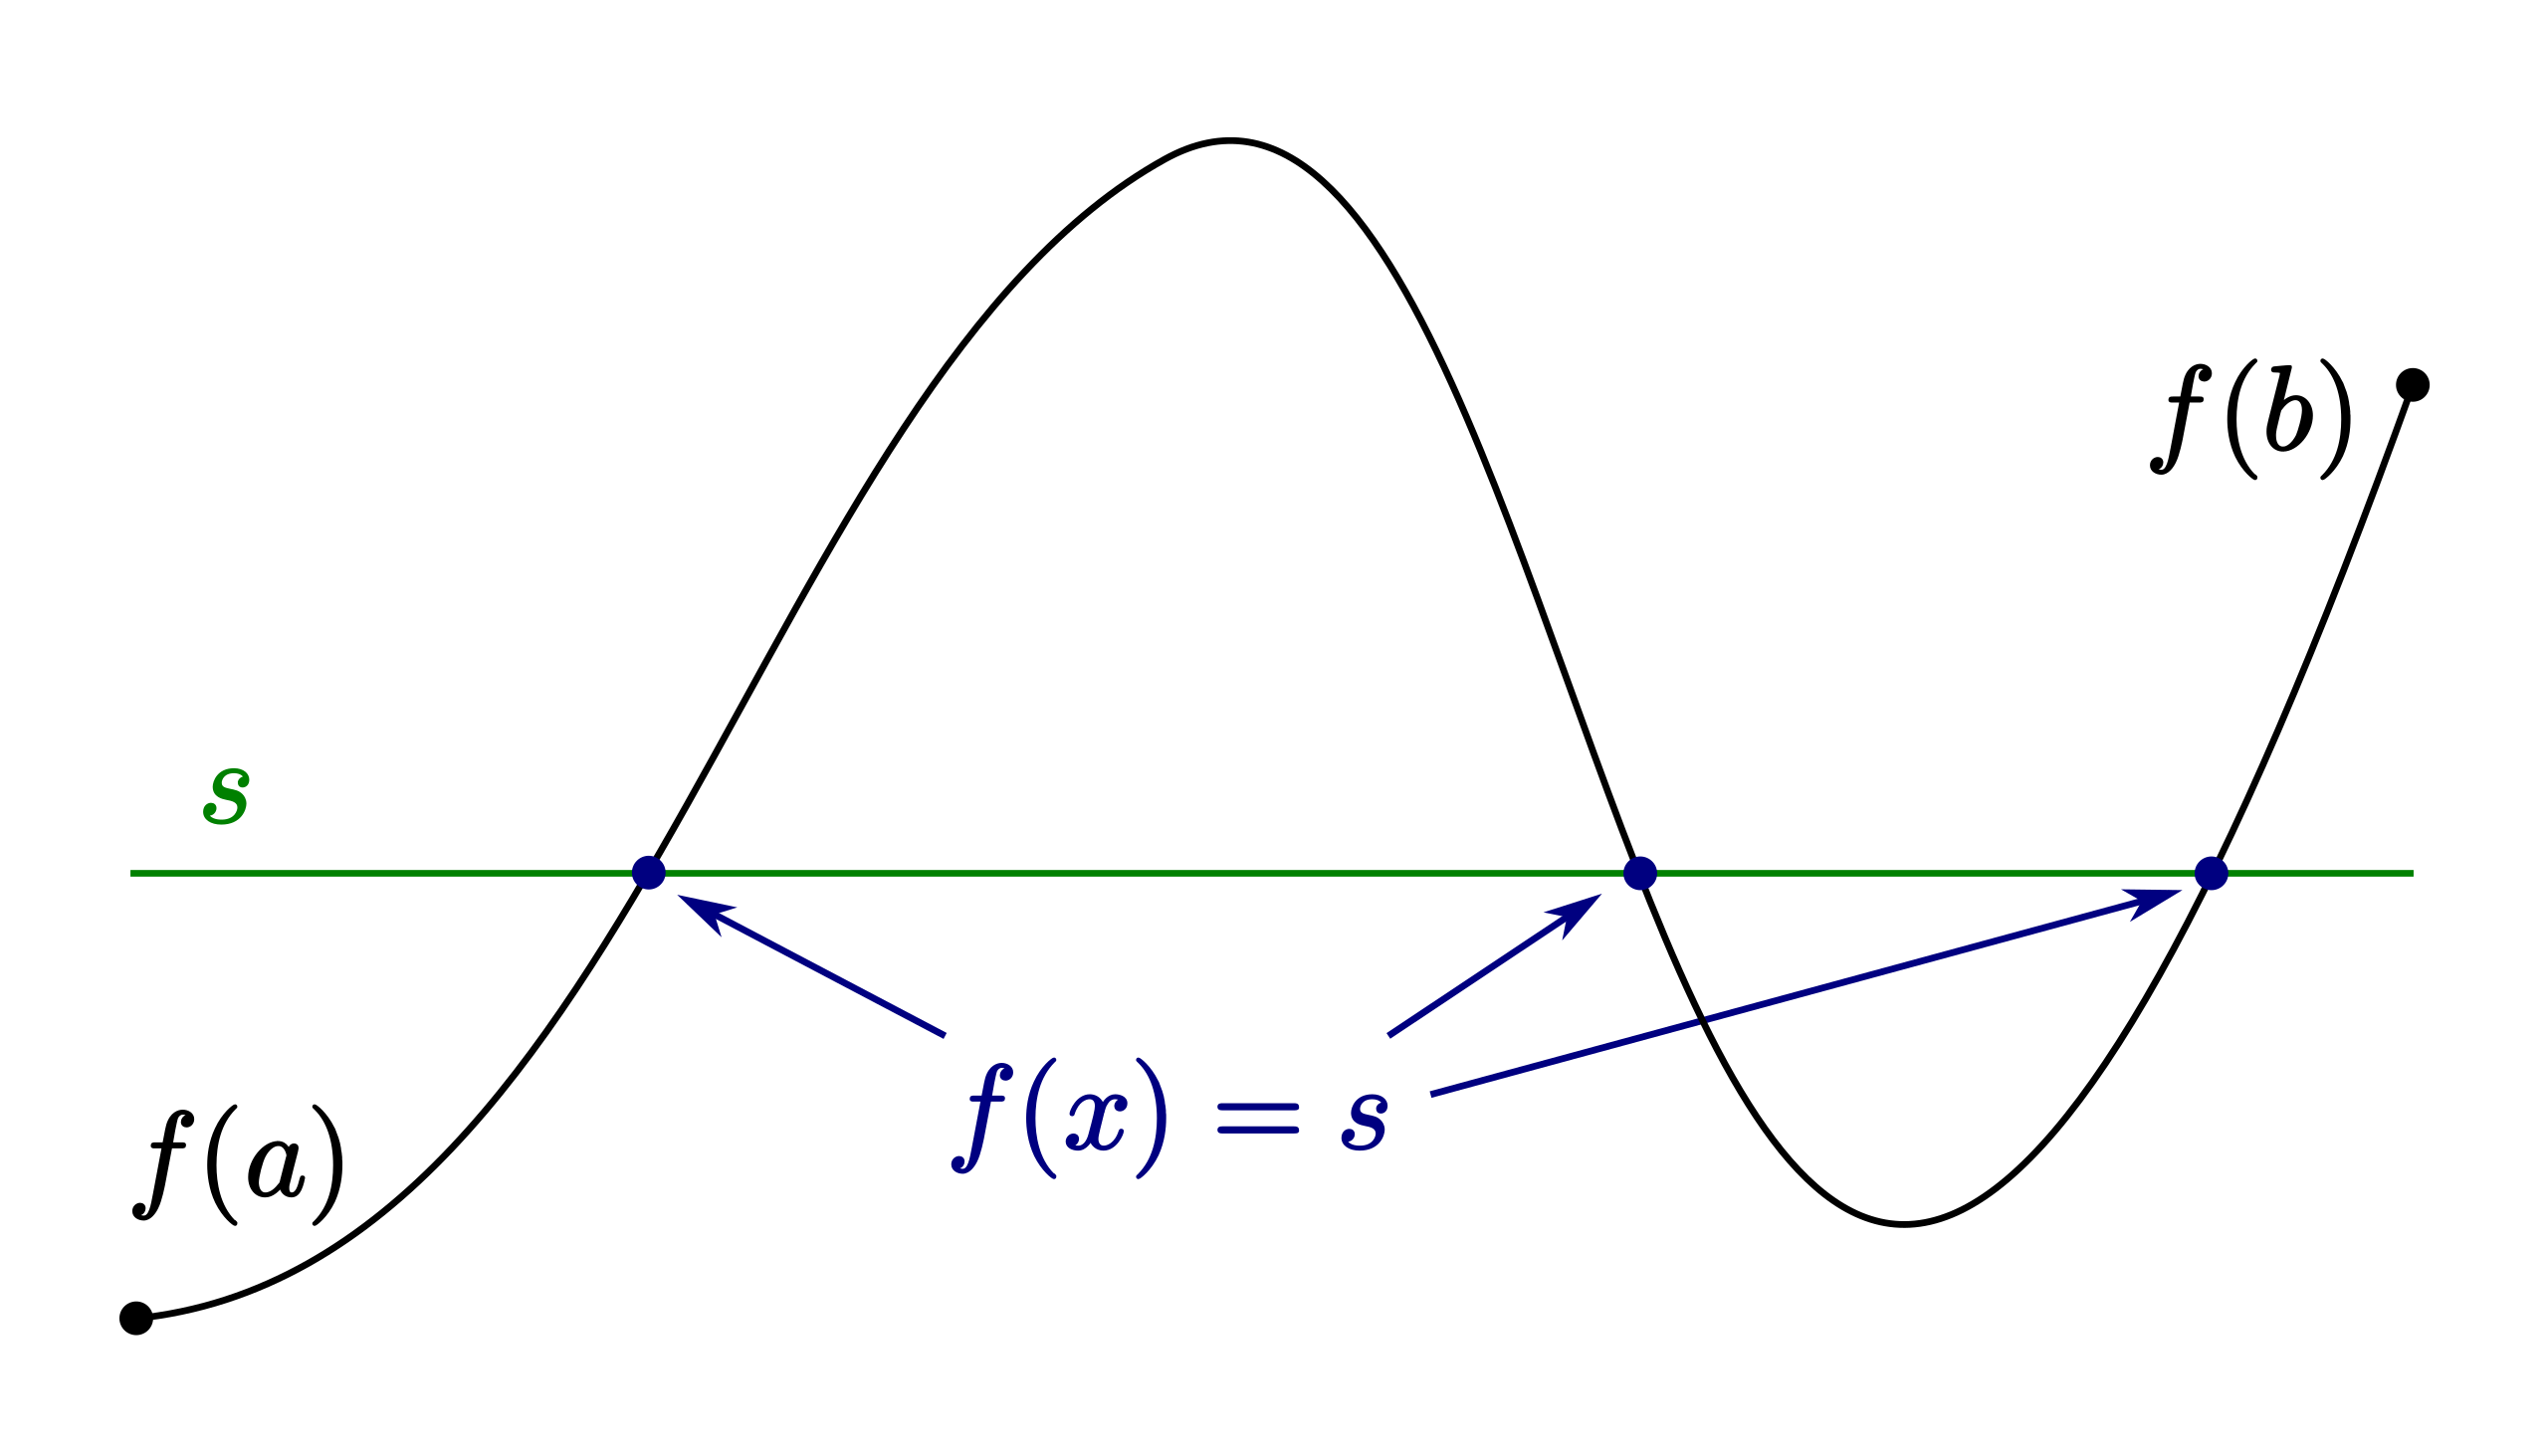
\includegraphics[width=0.45\textwidth]{figures/ivt.png}
\end{figure}
\end{frame}

\begin{frame}
\frametitle{Intermediate value theorem}
Functions that are continuous on the interval [a,b] exhibit many useful properties. One powerful theorem concerning such functions is the \textbf{intermediate value theorem}. This method is useful for finding roots of such a function, i.e. a solution to our root finding problem. \\\vspace{5pt} 
The intermediate value theorem states that if $f$ is a continuous function
on the interval $[a,b]$,  then it takes on any value between
$f(a)$ and $f(b)$ at some point within the interval. In other words,
let $s$ be a number with $f(a) < s < f(b)$. Then there exists some
$x$ such that $f(x) = s$. \\
\vspace{10pt}
In this example, we see that for some value $f(a) < s < f(b)$, there are several such $x$ values that satisfy $f(x) = s$.
\begin{figure}
	\center
	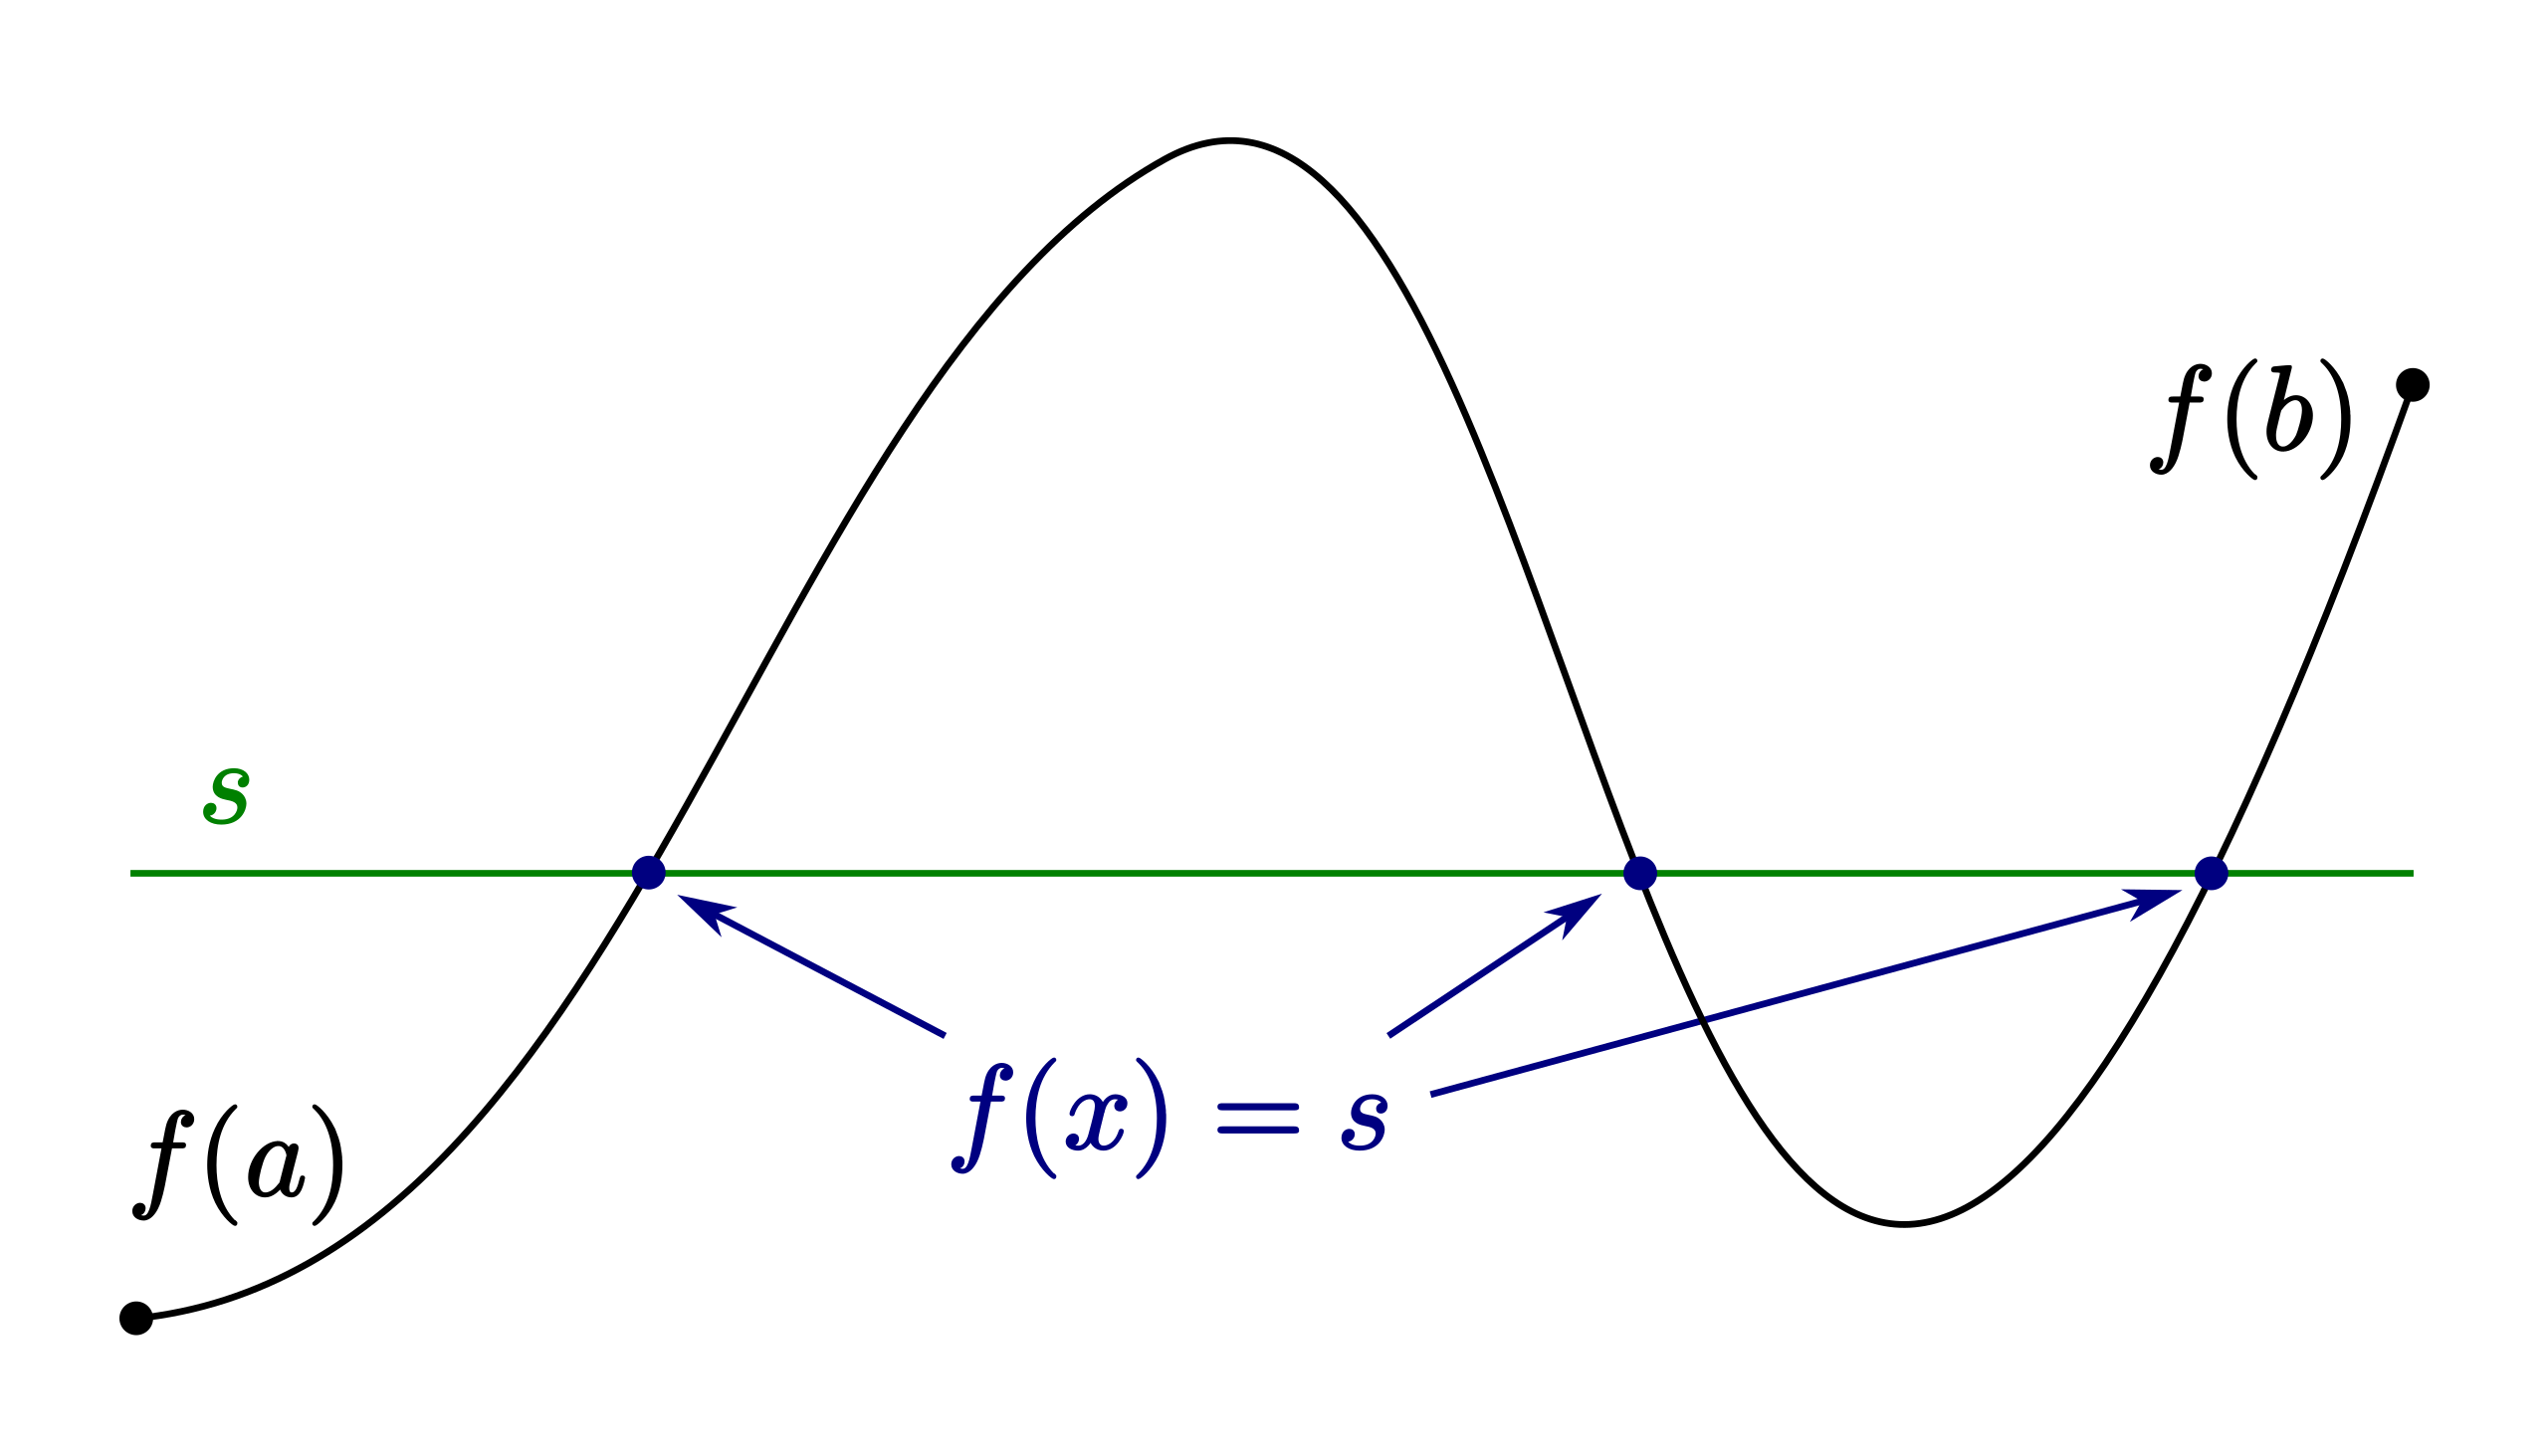
\includegraphics[width=0.45\textwidth]{figures/ivt.png}
\end{figure}
We can also note that if $s=0$, $f(a)$ is negative while $f(b)$ is positive, so $f(a)f(b)<0.$
\end{frame}


\begin{frame}
\frametitle{So now what?}
Now we know how to determine if our problem is well-posed. The question is how can we exploit this information to write some sort of scheme to systemically find the root(s) for us?
\end{frame}

\section{Incremental Search}
\begin{frame}
\frametitle{Incremental Search}
Think back to the bungee jump example. We observed that $f(x)$ changed sign on opposite sides of the root. In general, if $f(x)$ is real and continuous in the interval from $a$ to $b$ and $f(a)$ and $f(b)$ have opposite signs, that is,$f(a)f(b)<0$. Then there is at least one real root between $a$ and $b$. We showed this with the intermediate value theorem.
\\\vspace{0.25cm}
\begin{figure}
	\centering
	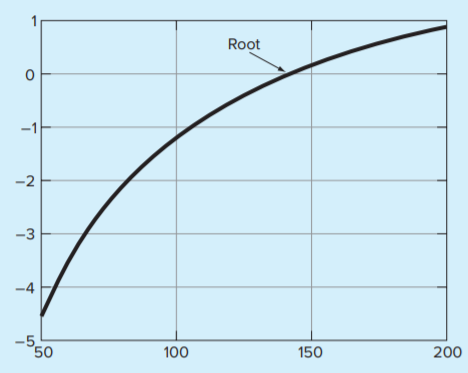
\includegraphics[width = 0.45\textwidth]{figures/BunjeeJumpGraph}
\end{figure}
%\\\vspace{0.25cm}
\textbf{Incremental search methods} capitalize on this observation by locating an interval (or bracket) where the function changes sign.
\end{frame}

\begin{frame}
\frametitle{Incremental Search}
\textbf{Incremental search methods} capitalize the observation that at least one root exists between $a$ and $b$ if $f(a)f(b)<0$. This method works by locating an interval where the function changes sign.  \\
\vspace{0.25cm}
The algorithm:
\begin{enumerate}
	\item Start with an initial range that contains the root, and subdivide it into several smaller sub-ranges. We will do an example with 4 sub-ranges.

\end{enumerate}
\begin{figure}
	\centering
	\includegraphics[width = 0.85\textwidth]{figures/incremental1}
\end{figure}
\end{frame}

\begin{frame}
\frametitle{Incremental Search}
Incremental search methods capitalize on this observation that at least one root exists between $a$ and $b$ if $f(a)f(b)<0$. This method works by locating an interval where the function changes sign.  \\
\vspace{0.25cm}
The algorithm:
\begin{enumerate}
	\item Start with an initial range that contains the root, and subdivide it into several smaller sub-ranges. We will do an example with 4 sub-ranges.
	\item Look inside each sub-range one by one for the root. When the sub-range containing the root is identified, choose the end of the range as the guess.
\end{enumerate}
\begin{figure}
	\centering
	\includegraphics[width = 0.85\textwidth]{figures/incremental1}
\end{figure}
\end{frame}

\begin{frame}
\frametitle{Incremental Search}
Incremental search methods capitalize on this observation that at least one root exists between $a$ and $b$ if $f(a)f(b)<0$. This method works by locating an interval where the function changes sign.  \\
\vspace{0.25cm}
The algorithm:
\begin{enumerate}
	\item Start with an initial range that contains the root, and subdivide it into several smaller sub-ranges. We will do an example with 4 sub-ranges.
	\item Look inside each sub-range one by one for the root. When the sub-range containing the root is identified, choose the end of the range as the guess.
	\item Evaluate the error of your guess. If it is too big, start back at step 1. 
\end{enumerate}
\begin{figure}
	\centering
	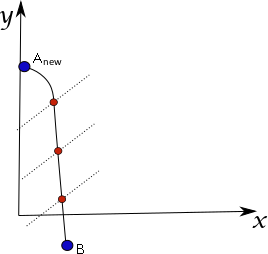
\includegraphics[width = 0.35\textwidth]{figures/incremental2}
\end{figure}
\end{frame}

\begin{frame}
\frametitle{Incremental Search}
Incremental search methods capitalize on this observation that at least one root exists between $a$ and $b$ if $f(a)f(b)<0$. This method works by locating an interval where the function changes sign.  \\
\vspace{0.25cm}
The algorithm:
\begin{enumerate}
	\item Start with an initial range that contains the root, and subdivide it into several smaller sub-ranges. We will do an example with 4 sub-ranges.
	\item Look inside each sub-range one by one for the root. When the sub-range containing the root is identified, choose the end of the range as the guess.
	\item Evaluate the error of your guess. If it is too big, start back at step 1. 
\end{enumerate}
\begin{figure}
	\centering
	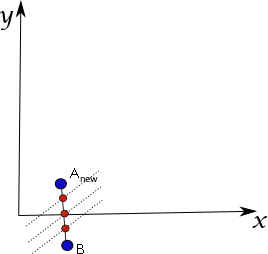
\includegraphics[width = 0.35\textwidth]{figures/incremental3}
\end{figure}
\end{frame}

\begin{frame}
\frametitle{Incremental Search}
Incremental search methods capitalize on this observation that at least one root exists between $a$ and $b$ if $f(a)f(b)<0$. This method works by locating an interval where the function changes sign.  \\
\vspace{0.25cm}
The algorithm:
\begin{enumerate}
	\item Start with an initial range that contains the root, and subdivide it into several smaller sub-ranges. We will do an example with 4 sub-ranges.
	\item Look inside each sub-range one by one for the root. When the sub-range containing the root is identified, choose the end of the range as the guess.
	\item Evaluate the error of your guess. If it is too big, start back at step 1. 
\end{enumerate}
\begin{figure}
	\centering
	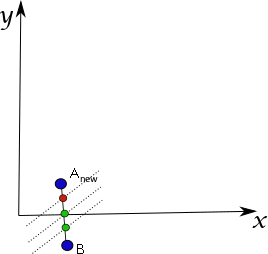
\includegraphics[width = 0.35\textwidth]{figures/incremental4}
\end{figure}
\end{frame}

\begin{frame}
\frametitle{Limits of the Incremental Search Method}
One potential problem with using the Incremental search method is the choice of increment length.
\begin{itemize}
	\item if the length is too small, the search can be very time consumming.
	\item if the length is too long, closely spaced roots might be missed. 
\end{itemize}
These problems are compounded by the possibility of multiple (double) roots.
\begin{figure}
	\centering
	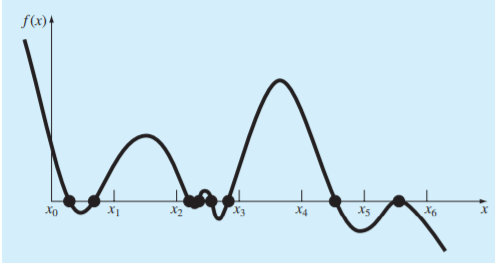
\includegraphics[width = 0.6\textwidth]{figures/fail}
\end{figure}

\end{frame}

\section{Bisection method}

\begin{frame}
\frametitle{Bisection method}
\begin{itemize}
	\item The Bisection method is a variation of the incremental search method in which the interval is always divided in half. \\
	\item If a function changes sign over the interval, the function at the midpoint is evaluated. \\
	\item The root is then determined to lie in the interval where the sign change occurs.\\
	\item That subinterval becomes the new interval for the next iteration.
	\item The process is repeated until the root is known to a required precision.
\end{itemize}
\end{frame}


\begin{frame}
\frametitle{Root is in interval}
Let's go back to that bungee jumping example. We can see that the function changes sign between values of 50 and 200. The plot obviously suggests better initial guesses, say 140 and 150, but let’s assume we don’t have the benefit of the plot and we made a conservative guess for our interval.So our initial estimate of the root $x_r$ lies at the midpoint of the interval
$$ x_r = \frac{50+200}{2} = 125 $$
\begin{figure}
\center
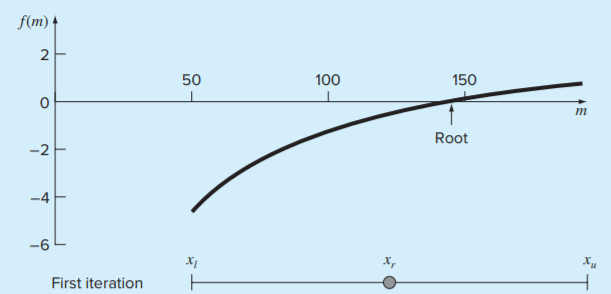
\includegraphics[width=0.7\textwidth]{figures/bracket.png}
\end{figure}
\end{frame}

\begin{frame}
\frametitle{Root is in interval}
\begin{figure}
	\center
	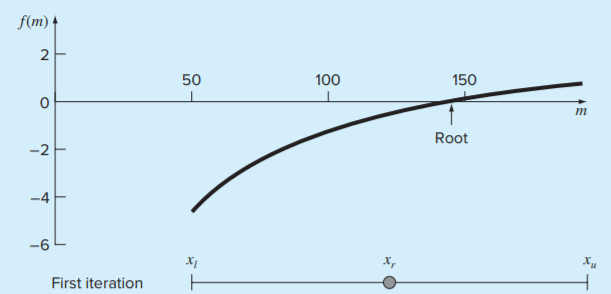
\includegraphics[width=0.7\textwidth]{figures/bracket.png}
\end{figure}
Next we compute the product of the function value at the lower bound and at the midpoint:
$$f(50)f(125) = −4.579*−0.409 = 1.871 > 0$$
which is greater than zero, and hence no sign change occurs between the lower bound and the midpoint. Consequently, the root must be located in the upper interval between 125 and 200. Therefore, we create a new interval by redefining the lower bound as 125.
\end{frame}

\begin{frame}
\frametitle{Bisect}
At this point, the new interval extends from $x_l = 125$ to $x_u = 200$. A revised root estimate can then be calculated as
$$ x_r = \frac{125+200}{2} = 162.5$$
\begin{figure}
\center
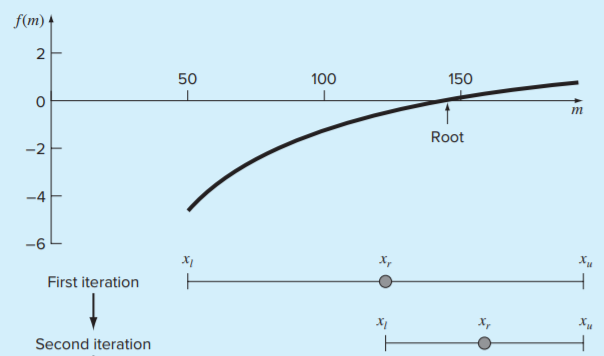
\includegraphics[width=0.7\textwidth]{figures/bracket2.png}
\end{figure}
\end{frame}

\begin{frame}
\frametitle{Bisect}
\begin{figure}
	\center
	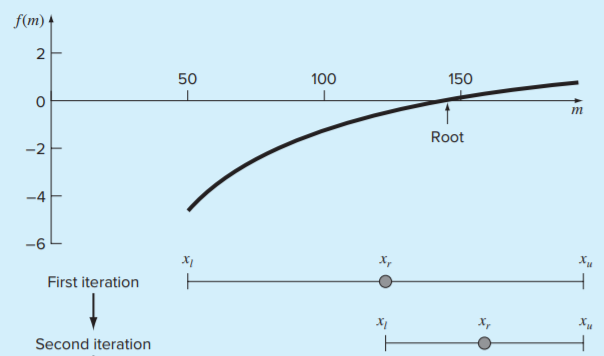
\includegraphics[width=0.7\textwidth]{figures/bracket2.png}
\end{figure}
Compute the product of the function value at the lower bound and at the midpoint:
$$f(125)f(162.5) = −0.409*0.359 = −0.147 < 0$$
Which is less than zero, there's a sign change between the lower bound and the midpoint. Therefore the root is located in the lower interval between 125 and 162.5. So we create a new interval by redefining the upper bound as 162.5.  
\end{frame}

\begin{frame}
\frametitle{Bisect}
\begin{figure}
	\center
	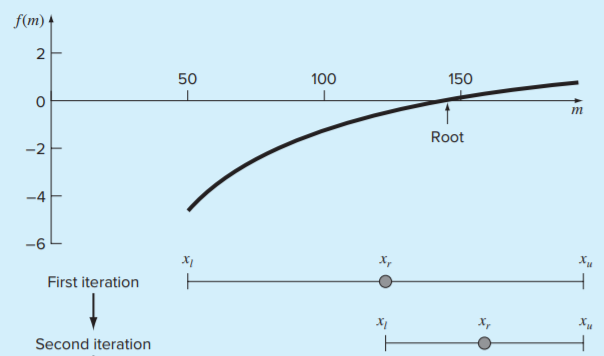
\includegraphics[width=0.7\textwidth]{figures/bracket2.png}
\end{figure}
Evaluate the \textit{percent relative error} 
$$ |\epsilon_a| = |\frac{x_r^{new}-x_r^{old}}{x_r^{new}}| $$
\end{frame}

\begin{frame}
\frametitle{Bisect}
\begin{figure}
\center
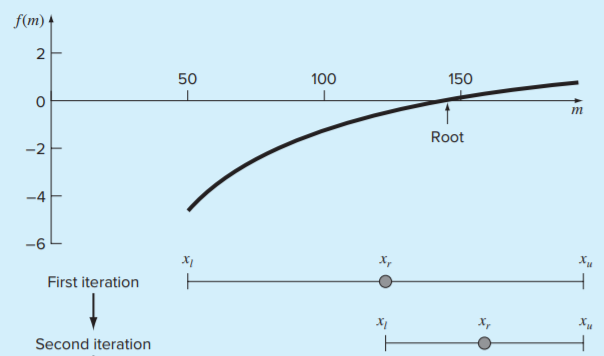
\includegraphics[width=0.7\textwidth]{figures/bracket2.png}
\end{figure}
Evaluate the \textit{percent relative error} 
$$ |\epsilon_a| = |\frac{162.5 - 125}{162.5}| \approx 23\% $$
If this is larger than your tolerance, continue the bisection algorithm.
\end{frame}

\begin{frame}
\frametitle{Bisect}
At this point, the new interval extends from $x_l = 125$ to $x_u = 162.5$. A revised root estimate can then be calculated as
$$ x_r = \frac{125+162.5}{2} = 143.75$$
\begin{figure}
\center
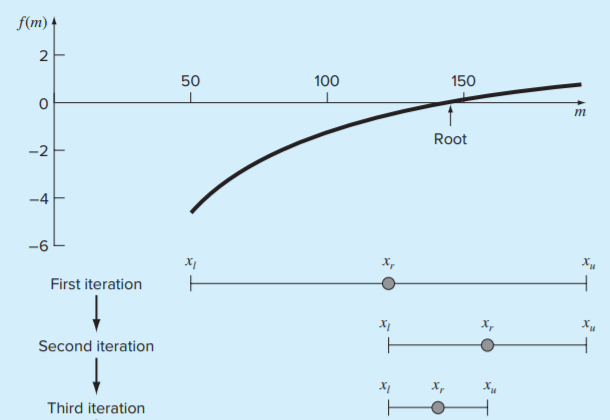
\includegraphics[width=0.7\textwidth]{figures/bracket3.png}
\end{figure}
\end{frame}


\begin{frame}
\frametitle{Bisect}
\begin{figure}
	\center
	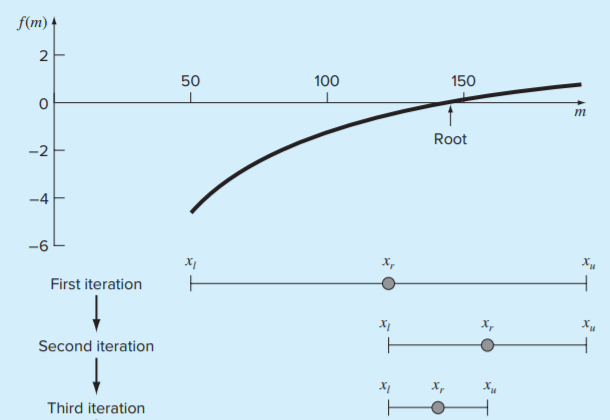
\includegraphics[width=0.7\textwidth]{figures/bracket3.png}
\end{figure}
Compute the product of the function value at the lower bound and at the midpoint:
$$f(125)f(143.75) = -0.409*0.021 = -.009 $$ 
Which is less than zero, there's a sign change between the lower bound and the midpoint. Therefore the root is located in the lower interval between 125 and 143.75. So we create a new interval by redefining the upper bound as 143.75.
\end{frame}

\begin{frame}
\frametitle{Bisect}
\begin{figure}
	\center
	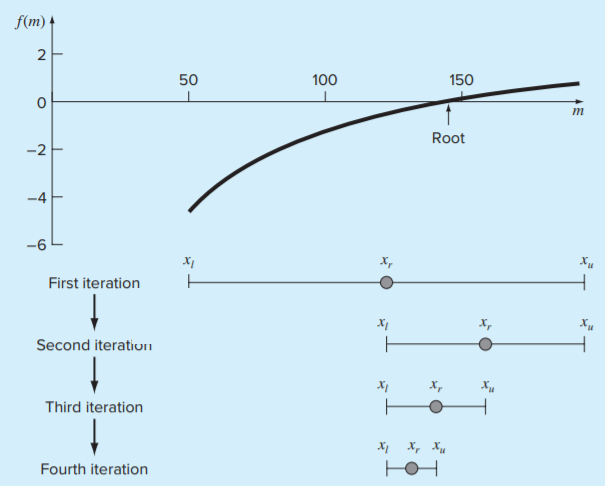
\includegraphics[width=0.65\textwidth]{figures/bracket4.png}
\end{figure}
Evaluate the \textit{percent relative error} 
$$ |\epsilon_a| = |\frac{143.75-162.5}{143.75}| \approx 13\%$$ 
If this is bigger than your tolerance, bisect.
\end{frame}


\begin{frame}[shrink=10]
\frametitle{Bisection algorithm}
\vspace{1cm}
\begin{enumerate}
\item specify a bracket $[a,b]$ that you think contains the root \\ \vspace{3pt}
\item evaluate $f(a)$ and $f(b)$ \\\vspace{3pt}
\item if $f(a)f(b) < 0.0$ then you have at least one root \\\vspace{3pt}
\item compute the midpoint within the interval, $c = \frac{1}{2}(a
+ b)$ \\\vspace{3pt}
\item check one of the new half-intervals for the root, $f(a)f(c) < 0.0$ \\\vspace{3pt}
\item if found, then set $b = c$ and start at step 2 - 
otherwise set $a = c$ and start at step 2 \\\vspace{3pt}
\item exit the algorithm if the percent relative error is less than your tolerance \\\vspace{3pt}
\end{enumerate}
\end{frame}

\begin{frame}
\frametitle{Beware multiple roots}
There are many cases where bisection method would fail even for a continuous
function.
\begin{figure}
\center
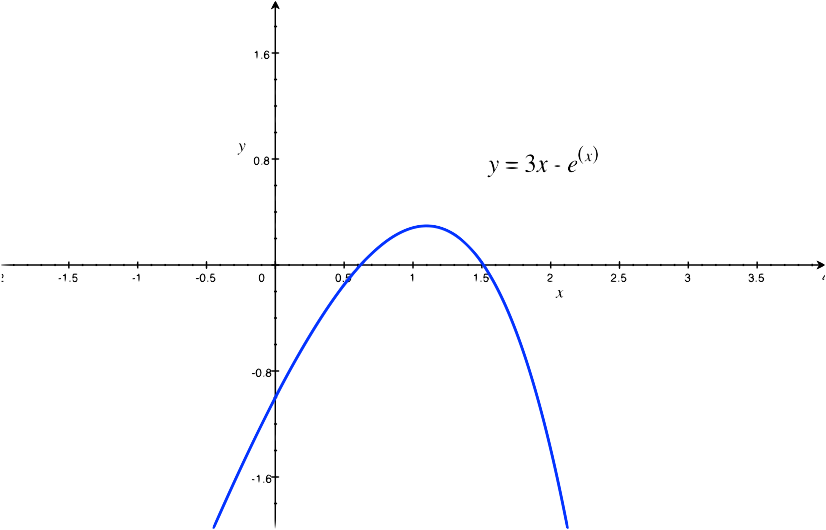
\includegraphics[width=0.75\textwidth]{figures/doubleroot.png}
\end{figure}
\end{frame}

\begin{frame}
\frametitle{Sign-off activity}
In computer science, pseudocode is a plain language description of the steps in an algorithm or another system. Pseudocode often uses structural conventions of a normal programming language but is intended for human reading rather than machine reading-so the syntax doesn't need to be exactly right. Think of it as a pen and paper rough-draft of the code you will write. \\\vspace{10pt} 
Write a pseudocode for the Bisection method based on the steps outlined in the algorithm slide (slide 54).
\\\vspace{10pt} 
When you are finished, post your draft in the discussion board \textbf{Bisection Pseudocode}. 
\end{frame}

\end{document}
